\ifdefined\included
\else
\documentclass[a4paper,11pt,twoside]{StyleThese}
\usepackage{amsmath,amssymb, amsthm}             % AMS Math
\usepackage[T1]{fontenc}
\usepackage[utf8x]{inputenc}
\usepackage{babel}
\usepackage{datetime}

\usepackage{silence}

\WarningFilter{minitoc(hints)}{W0023}
\WarningFilter{minitoc(hints)}{W0028}
\WarningFilter{minitoc(hints)}{W0030}

\usepackage{lmodern}
\usepackage{tabularx}
%\usepackage{tabular}
\usepackage{multirow}
\usepackage{xspace}

\usepackage{hhline}
\usepackage[left=1.5in,right=1.3in,top=1.1in,bottom=1.1in,includefoot,includehead,headheight=13.6pt]{geometry}
\renewcommand{\baselinestretch}{1.05}

% Table of contents for each chapter

\usepackage[nottoc, notlof, notlot]{tocbibind}
\usepackage{minitoc}
\setcounter{minitocdepth}{2}
\mtcindent=15pt
% Use \minitoc where to put a table of contents

\usepackage{aecompl}

% Glossary / list of abbreviations

\usepackage[intoc]{nomencl}
\iftoggle{ThesisInEnglish}{%
\renewcommand{\nomname}{Glossary}
}{ %
\renewcommand{\nomname}{Liste des Abréviations}
}

\usepackage{etoolbox}
\renewcommand\nomgroup[1]{%
  \item[\bfseries
  \ifstrequal{#1}{A}{Number Sets}{%
  \ifstrequal{#1}{G}{Agents Beliefs and Action Models}{%
  \ifstrequal{#1}{N}{Navigation}{%
  \ifstrequal{#1}{O}{Ontology}{%
  \ifstrequal{#1}{R}{Referring Expression Generation}{%
  \ifstrequal{#1}{Z}{Controllable and Uncontrollable Agents Task Planning}{}}}}}}%
]}

\makenomenclature



% My pdf code

\usepackage{ifpdf}

\ifpdf
  \usepackage[pdftex]{graphicx}
  \DeclareGraphicsExtensions{.jpg}
  \usepackage[pagebackref,hyperindex=true]{hyperref}
  \usepackage{tikz}
  \usetikzlibrary{arrows,shapes,calc}
\else
  \usepackage{graphicx}
  \DeclareGraphicsExtensions{.ps,.eps}
  \usepackage[dvipdfm,pagebackref,hyperindex=true]{hyperref}
\fi

\graphicspath{{.}{images/}}

%% nicer backref links. NOTE: The flag ThesisInEnglish is used to define the
% language in the back references. Read more about it in These.tex

\iftoggle{ThesisInEnglish}{%
\renewcommand*{\backref}[1]{}
\renewcommand*{\backrefalt}[4]{%
\ifcase #1 %
(Not cited.)%
\or
(Cited in page~#2.)%
\else
(Cited in pages~#2.)%
\fi}
\renewcommand*{\backrefsep}{, }
\renewcommand*{\backreftwosep}{ and~}
\renewcommand*{\backreflastsep}{ and~}
}{%
\renewcommand*{\backref}[1]{}
\renewcommand*{\backrefalt}[4]{%
\ifcase #1 %
(Non cité.)%
\or
(Cité en page~#2.)%
\else
(Cité en pages~#2.)%
\fi}
\renewcommand*{\backrefsep}{, }
\renewcommand*{\backreftwosep}{ et~}
\renewcommand*{\backreflastsep}{ et~}
}

% Links in pdf
\usepackage{color}
\definecolor{linkcol}{rgb}{0,0,0.4} 
\definecolor{citecol}{rgb}{0.5,0,0} 
\definecolor{linkcol}{rgb}{0,0,0} 
\definecolor{citecol}{rgb}{0,0,0}
% Change this to change the informations included in the pdf file

\hypersetup
{
bookmarksopen=true,
pdftitle="Planning For Both Robot and Human: Anticipating and Accompanying Human Decisions",
pdfauthor="Guilhem BUISAN", %auteur du document
pdfsubject="Thèse", %sujet du document
%pdftoolbar=false, %barre d'outils non visible
pdfmenubar=true, %barre de menu visible
pdfhighlight=/O, %effet d'un clic sur un lien hypertexte
colorlinks=true, %couleurs sur les liens hypertextes
pdfpagemode=None, %aucun mode de page
pdfpagelayout=SinglePage, %ouverture en simple page
pdffitwindow=true, %pages ouvertes entierement dans toute la fenetre
linkcolor=linkcol, %couleur des liens hypertextes internes
citecolor=citecol, %couleur des liens pour les citations
urlcolor=linkcol %couleur des liens pour les url
}

% definitions.
% -------------------

\setcounter{secnumdepth}{3}
\setcounter{tocdepth}{2}

% Some useful commands and shortcut for maths:  partial derivative and stuff

\newcommand{\pd}[2]{\frac{\partial #1}{\partial #2}}
\def\abs{\operatorname{abs}}
\def\argmax{\operatornamewithlimits{arg\,max}}
\def\argmin{\operatornamewithlimits{arg\,min}}
\def\diag{\operatorname{Diag}}
\newcommand{\eqRef}[1]{(\ref{#1})}

\usepackage{rotating}                    % Sideways of figures & tables
%\usepackage{bibunits}
%\usepackage[sectionbib]{chapterbib}          % Cross-reference package (Natural BiB)
%\usepackage{natbib}                  % Put References at the end of each chapter
                                         % Do not put 'sectionbib' option here.
                                         % Sectionbib option in 'natbib' will do.
\usepackage{fancyhdr}                    % Fancy Header and Footer

% \usepackage{txfonts}                     % Public Times New Roman text & math font
  
%%% Fancy Header %%%%%%%%%%%%%%%%%%%%%%%%%%%%%%%%%%%%%%%%%%%%%%%%%%%%%%%%%%%%%%%%%%
% Fancy Header Style Options

\pagestyle{fancy}                       % Sets fancy header and footer
\fancyfoot{}                            % Delete current footer settings

%\renewcommand{\chaptermark}[1]{         % Lower Case Chapter marker style
%  \markboth{\chaptername\ \thechapter.\ #1}}{}} %

%\renewcommand{\sectionmark}[1]{         % Lower case Section marker style
%  \markright{\thesection.\ #1}}         %

\fancyhead[LE,RO]{\bfseries\thepage}    % Page number (boldface) in left on even
% pages and right on odd pages
\fancyhead[RE]{\bfseries\nouppercase{\leftmark}}      % Chapter in the right on even pages
\fancyhead[LO]{\bfseries\nouppercase{\rightmark}}     % Section in the left on odd pages

\let\headruleORIG\headrule
\renewcommand{\headrule}{\color{black} \headruleORIG}
\renewcommand{\headrulewidth}{1.0pt}
\usepackage{colortbl}
\arrayrulecolor{black}

\fancypagestyle{plain}{
  \fancyhead{}
  \fancyfoot{}
  \renewcommand{\headrulewidth}{0pt}
}

%\usepackage{MyAlgorithm}
%\usepackage[noend]{MyAlgorithmic}
\usepackage{algorithm}
\usepackage[noend]{algpseudocode}
\usepackage{comment}
\usepackage[ED=EDSYS-Robo, Ets=INSA]{tlsflyleaf}
%%% Clear Header %%%%%%%%%%%%%%%%%%%%%%%%%%%%%%%%%%%%%%%%%%%%%%%%%%%%%%%%%%%%%%%%%%
% Clear Header Style on the Last Empty Odd pages
\makeatletter

\def\cleardoublepage{\clearpage\if@twoside \ifodd\c@page\else%
  \hbox{}%
  \thispagestyle{empty}%              % Empty header styles
  \newpage%
  \if@twocolumn\hbox{}\newpage\fi\fi\fi}

\makeatother
 
%%%%%%%%%%%%%%%%%%%%%%%%%%%%%%%%%%%%%%%%%%%%%%%%%%%%%%%%%%%%%%%%%%%%%%%%%%%%%%% 
% Prints your review date and 'Draft Version' (From Josullvn, CS, CMU)
\newcommand{\reviewtimetoday}[2]{\special{!userdict begin
    /bop-hook{gsave 20 710 translate 45 rotate 0.8 setgray
      /Times-Roman findfont 12 scalefont setfont 0 0   moveto (#1) show
      0 -12 moveto (#2) show grestore}def end}}
% You can turn on or off this option.
% \reviewtimetoday{\today}{Draft Version}
%%%%%%%%%%%%%%%%%%%%%%%%%%%%%%%%%%%%%%%%%%%%%%%%%%%%%%%%%%%%%%%%%%%%%%%%%%%%%%% 

\newenvironment{maxime}[1]
{
\vspace*{0cm}
\hfill
\begin{minipage}{0.5\textwidth}%
%\rule[0.5ex]{\textwidth}{0.1mm}\\%
\hrulefill $\:$ {\bf #1}\\
%\vspace*{-0.25cm}
\it 
}%
{%

\hrulefill
\vspace*{0.5cm}%
\end{minipage}
}

\let\minitocORIG\minitoc
\renewcommand{\minitoc}{\minitocORIG \vspace{1.5em}}

\usepackage{multirow}
%\usepackage{slashbox}

\newenvironment{bulletList}%
{ \begin{list}%
	{$\bullet$}%
	{\setlength{\labelwidth}{25pt}%
	 \setlength{\leftmargin}{30pt}%
	 \setlength{\itemsep}{\parsep}}}%
{ \end{list} }

\theoremstyle{definition}
\newtheorem{definition}{Definition}
\renewcommand{\epsilon}{\varepsilon}

% centered page environment

\newenvironment{vcenterpage}
{\newpage\vspace*{\fill}\thispagestyle{empty}\renewcommand{\headrulewidth}{0pt}}
{\vspace*{\fill}}

\usepackage{tablefootnote}

\theoremstyle{plain}
\newtheorem{constraint}{Constraint}[section]

\algnewcommand\algorithmicforeach{\textbf{for each}}
\algnewcommand\algorithmicin{\textbf{in}}
\algdef{S}[FOR]{ForEach}[2]{\algorithmicforeach\ #1\ \algorithmicin\ #2\ \algorithmicdo}

\usepackage{listings}
\lstdefinestyle{customPlan}{
  language=C,
  commentstyle=\itshape\color{green!25!black},
}
\usepackage{pdfpages}

\sloppy
\begin{document}
\setcounter{chapter}{3} %% Numéro du chapitre précédent ;)
\dominitoc
\faketableofcontents
\fi

\chapter{Emulating the human planning process during task planning}
\minitoc

\section{Introduction}
In the previous chapter we successfully integrated a verbal communication planner into a multi agents task planner. This allows to avoid many plan failures, repair actions or unefficiency during the execution. Although we saw that this approach needs a task planner able to maintain one set of beliefs per agent during the planning process, the planner used was only allocating task to the human without considering that the human is not aware of the plan generated.

In this chapter we propose a first step to tackle this issue. We present a novel approach, where, instead of planning and allocating tasks to the human without planning for any plan communication, use a human action model to predict possible human actions, considering their reaction and own planning process.

First, we describe our approach and introduce the notations used in this chapter before detailing the planning process. Then, we demonstrate the planner capabilities on two example situations. Finally, we present a task inspired from psychology which is particularly interesting for HRI and has never been tackled in robotics yet, and we show how our planner has been integrated in a fully functional robotic architecture dedicated to this new task.

\section{Description}
We separate agents involved in a given task into two categories: the controllable agent (\textit{i.e.} the robot) for which the planner needs to select the best course of actions to generate a plan; and the uncontrollable agent (\textit{i.e.} the human) on whom the planner has no direct control but, still, has a representation of their decision and action models. The two agent types are fundamentally different: (1) the robot is controllable since the process is run by the robot, (2) the human agent is not controllable since the process can only "speculate" on her/his decisions and actions, but can model that the robot actions can still influence them, (3) the two agents are not equivalent, the robot agent role is to help, assist and facilitate human and to synthesize pertinent, legible and acceptable behavior.
We want to devise a planner allowing the controllable agent to plan for its actions while anticipating the decisions, actions and reactions of the uncontrollable agent. Moreover, we want the planner to be able to generate plans where the robot actions elicit situations calling for human decision, action and reaction, thus creating and anticipating collaboration and interaction.

This problem may be seen as a classical non deterministic planning problem, but enriched with the ability of the robot to model the actions, beliefs and decision process of the human. Thus, we have to consider distinct action models, beliefs and execution streams for each of the agents involved. Doing so with classical STRIPS-style planning approaches would lead to an intractable search space. Therefore, we chose to use HTN planning for both the controllable and uncontrollable agents. HTN planning aims at decomposing abstract tasks into atomic primitive tasks by choosing from a list of available context-dependent refinements for each abstract task, ensuring that preconditions and effects of refined primitives tasks are respected throughout the created plan. Similarly to HATP~\cite{sebastiani2017dealing}, our planner elaborates a plan with several streams of actions each associated to an agent involved in the task. But while in HATP, all the streams are built starting from on initial root node corresponding to a shared goal of all agents, our planner starts from multiple initial root nodes corresponding to the decision process of the different agents.

\paragraph{\bf Beliefs:}
Let $\statespace$ be the set of all possible world states, we call beliefs of an agent $\agent$ the state $\worldstate_{\agent} \in \statespace$ in which this agent thinks the world is in. It is important to note that the state of the controllable agent is assumed to be the world state estimation for the planner, as we consider the planner as being part of the controllable agent.

\paragraph{\bf Action models:}
We represent the action model of an agent $\agent$ as $\actionmodel_{\agent} = \langle \operators_{\agent}, \abstracttasks_{\agent}, \methods_{\agent} \rangle$ where $\operators_{\agent}$ are the primitive tasks (\textit{i.e.} operators, actions) that the agent $\agent$ can perform, $\abstracttasks_{\agent}$ the set of abstract tasks and $\methods_{\agent}$ are the methods (\textit{i.e.} decompositions) describing how an agent $\agent$ can perform an abstract task though a refinement process.

\paragraph{\bf Agents agendas and plans:}
An agenda $\agenda_{\agent}$ and a plan $\plan_{\agent}$ (this agent only stream of actions) are defined for each agent $\agent$. The agenda $\agenda_{\agent}$ is a list of tasks (abstract or primitive) having to be performed by the agent. The plan $\plan_{\agent}$ is a list of primitive tasks, built from the agenda, which the agent has to perform.
Coordination between agent plans are represented by causal links between streams which correspond to effects of agents actions on the beliefs states of the other agents. 

\paragraph{\bf Agent triggers:}
We then define for each agent $\agent$ a set of so-called \textit{trigger functions} $\triggerset_{\agent}$. These trigger functions aim at representing reactions of agents to certain situations (subsets of worlds states).

\paragraph{\bf Agents:}
Finally, we define an agent state as a tuple $\agentstate_{\agent} = \langle  \agenda_{\agent}, \plan_{\agent}, \worldstate_{\agent} \rangle$, and an agent as being $\agent = \langle \text{name}_{\agent}, \agentstate_{\agent}, \actionmodel_{\agent}, \triggerset_{\agent} \rangle$. Then we define two agent: the controllable one --- the \textit{robot} ---; and the uncontrollable one --- the \textit{human} ---. Let $\agentsstatesset$ be the set of all the possible agents states.

\section{Planning process}
The cooperative agents planning problem consists in two agents $\agents_{start}$ with their respective agenda filled with tasks to achieve and their beliefs about the current world. For the controllable agent, the beliefs correspond to the planner ground truth, for the uncontrollable agent, their beliefs need to be estimated, through, for example, situation assessment component~\cite{milliez2014framework, lemaignan2018underworlds}.

The result is a robot conditional plan $\policy$ being a tree of alternating robot and human primitive tasks. Any path from the root to the leaves is a feasible sequence of primitive tasks (\textit{i.e.} each primitive task application leads to a state where the following one is applicable) leading to a state where all the controllable agents agenda are empty.

To solve such a problem we need to augment the search space from world states $\statespace$ only to all the agents states considered by the planner $\agentsstates$, with their agenda, plan and beliefs. The exploration starts with $\agentsstates^{start}$ and consecutively applies operators associated to the robot and to the human, leading to new agents states $\agentsstates^{i}$ until the controllable agent has an empty agenda: $\agenda_{robot} = ()$.

\subsection{Action models restriction}
Considering the definitions above, for any agent $\agent$ the operators are defined as functions: $\operators \ni o: \agentsstatesset \rightarrow \agentsstatesset \cup \bot$ which produce new agents state, being the effect of the application of the primitive task, or \textit{false} if the task is not applicable.
Methods are defined as tuple, containing an abstract task and a decomposition function: $\methods \ni m = \langle \alpha, \delta \rangle$ with $\alpha \in \abstracttasks$ and $\delta: \agentsstatesset \rightarrow (\operators \cup \abstracttasks)^n \cup () \cup \bot$ with $n \in \intset^*$, which, depending on agents states, decompose the abstract task returning a list of tasks (primitive or abstract), an empty list if the abstract task does not need to be decomposed, or \textit{false} if the task cannot be decomposed in the current state. Multiple methods can address the same abstract task, the goal of the HTN planner is then to choose the right one to create a plan.
Finally triggers function are defined as: $\triggerset \ni t: \agentsstatesset \rightarrow (\operators \cup \abstracttasks)^n \cup ()$ with $n \in \intset^*$, returning a list of tasks to be inserted in an agent agenda as a reaction to specific agent states. 

However, some constraints on these functions must be respected.  Indeed, depending on whether the agent is controllable or not, their planning process will not take decisions based on the same information, and their action will not impact the world state in the same manner. We thus impose restrictions on what a function can read and write (writing means here having effects on agents states and is only in the case of primitive task functions) in the agents state. Then, the function constraints also depend on which agent is performing the action or making the decision (in method and trigger functions). When a function is applied we note \textit{self} the agent which executes it and \textit{other} the other agent. The rules for read and write access are given in Table~\ref{table:function_restrictions}. 
\begin{table}
\centering
\begin{tabular}{|c||c|c|} 
 \hline
 Agent type & Readable & Writable \\
 \hline
 Controllable & \begin{tabular}[c]{@{}l@{}}$\worldstate_{self}, \worldstate_{other},$ \\ $\plan_{self}, \plan_{other}$ (1)\end{tabular} & \begin{tabular}[c]{@{}l@{}}$\worldstate_{self}, \worldstate_{other},$(2)\\ $\agenda_{self}, \agenda_{other}$ (3)\end{tabular}\\
 \hline
 Uncontrollable & $\worldstate_{self}, \plan_{self}$ (4) & $\worldstate_{self}, \worldstate_{other}, \agenda_{self}$ (5)\\
 \hline
\end{tabular}
\caption{Readable and writable elements (belief states, agenda, plan) of the agents state by method, primitive task and trigger functions.}
\label{table:function_restrictions}
\end{table}
\paragraph{(1)}During robot planning, the decision and the action can depend on the beliefs of the robot and on the planned estimated beliefs of the human. Moreover, the current partial plan of the robot and the anticipated plan of human one can also be used to make decisions.

\paragraph{(2)} The effects of robot actions obviously impact its own belief state (considered as the real world state by the planner), but also the beliefs of the human, for example, through their observation process and first order logic reasoning. More elaborate schemes to compute the effects can also be devised such as those described in~\cite{gharbi2015combining}.

\paragraph{(3)} Besides, a robot action can add a new task to the agenda of the human. This is to account for communication actions requesting the human to do something.

\paragraph{(4)} The human decisions and actions can only be done according to her own beliefs and partial plan. Indeed, we cannot add the robot ones as it is, or we would consider that the human estimation of the robot knowledge and past actions is always perfect. This would require a third type of agents, being the robot model as estimated by our estimation of the human. Here, we make the assumption that the human is a naive user, and thus, will not take their decision based on the estimated robot beliefs and past plan.

\paragraph{(5)}The effects of the human actions obviously impact their beliefs and the robot (planner) ones. Moreover, the human agenda could also be updated through, for example, a positive answer of a task request.
%\end{itemize}


\subsection{Exploration algorithm}
Our planner operates in a turn-taking scheme, based on the update of the agents beliefs states, the HTNs of the robot and the human are explored successively.

\begin{algorithm}[H]
\begin{algorithmic}[1]
\Function {SeekPlans}{$robot$, $human$}
\State $solutions \leftarrow$ an empty list of plans
\State $result \leftarrow \textsc{ExploreTree}(robot, human, solutions)$
\If {$result =$ failure} \Return failure \EndIf
\State \Return $solutions$
\EndFunction
\Statex
\Function {ExploreTree}{$r$, $h$, $solutions$}
\If {$\textsc{isEmpty}(\agenda_r)$}
	\State add the plan $\plan_r \cup \plan_h$ in $solutions$
	\State \Return success
\EndIf
\State $\lambda \leftarrow \textsc{Pop}(\agenda_r)$
\If{$\lambda \in \abstracttasks_r$}
	\State $isOneValid \leftarrow$ false
	\ForEach{$\langle \alpha, \delta \rangle$}{$\methods_r$ s.t. $\alpha = \lambda$}
		\State $decomposition \leftarrow \delta(\worldstate_r, \plan_r, \agenda_r, \worldstate_h, \plan_h, \agenda_h)$
		\If {$decomposition \neq \bot$}
			\State $r', h' \leftarrow \textsc{Copy}(r, h)$
			\State $\agenda_{r'} \leftarrow decomposition.\agenda_{r'}$
			\State $result \leftarrow \textsc{ExploreTree}(r', h', solutions)$
			\If {$result =$ success}
				$isOneValid \leftarrow$ true
			\EndIf
		\EndIf
	\EndFor
	\If {$isOneValid$} \Return success \EndIf
\EndIf
\If{$\lambda \in \operators_r$}
	\State $result \leftarrow \lambda(\worldstate_r, \plan_r, \agenda_r, \worldstate_h, \plan_h, \agenda_h)$
	\If {$result = \bot$}
		\Return failure
	\EndIf
	\State $r', h' \leftarrow \textsc{Copy}(r, h)$
	\State $\worldstate_{r'}, \agenda_{r'}, \worldstate_{h'}, \agenda_{h'} \leftarrow \textsc{Apply}(result)$
	\State $\plan_{r'} \leftarrow \plan_{r'}.\lambda$
	\State $\agenda_{r'}, \agenda_{h'} \leftarrow \textsc{ApplyTriggers}(\worldstate_{r'}, \plan_{r'}, \agenda_{r'}, \worldstate_{h'}, \plan_{h'}, \agenda_{h'})$
	\State $humanApplicableOperators \leftarrow \textsc{GetHumanApplicableOperators}(h')$
	\State $isOneValid \leftarrow$ false
	\ForEach{$o$}{$humanApplicableOperators$}
		\State $r'', h'' \leftarrow \textsc{Copy}(r', h')$
		\State $\worldstate_{r''}, \worldstate_{h''}, \agenda_{h''} \leftarrow \textsc{Apply}(o)$
		\State $\agenda_{r''}, \agenda_{h''} \leftarrow \textsc{ApplyTriggers}(\worldstate_{r''}, \plan_{r''}, \agenda_{r''}, \worldstate_{h''}, \plan_{h''}, \agenda_{h''})$
		\State $result \leftarrow \textsc{ExploreTree}(r'', h'', solutions)$
		\If {$result =$ success} $isOneValid \leftarrow$ true \EndIf
	\EndFor
	\If {$isOneValid$} \Return success \EndIf
\EndIf
\EndFunction
\end{algorithmic}
 \caption{Double HTN main exploration algorithm.}
  \label{alg:seek_plans}
\end{algorithm}

\begin{algorithm}[H]
\begin{algorithmic}[1]
\Function {GetHumanApplicableOperators}{$h$}
\State $solution \leftarrow ExploreApplicableOps(h)$
\If {$solution = ()$}
	\Return $(WAIT)$
\EndIf
\EndFunction
\Statex
\Function{ExploreApplicableOps}{$h$}
\If{$\textsc{isEmpty}(d_h)$}
	\Return $(IDLE)$
\EndIf
\State $\lambda \leftarrow \textsc{Pop}(\agenda_h)$
\If {$\lambda \in \abstracttasks_h$}
	\State $applicableOps \leftarrow$ an empty set of operators
	\ForEach{$\langle \alpha, \delta \rangle$}{$\methods_h$ s.t. $\alpha = \lambda$}
		\State $decomposition \leftarrow \delta(\worldstate_h, \plan_h)$
		\If {$decomposition \neq \bot$}
			\State $h' \leftarrow \textsc{Copy}(h)$
			\State $\agenda_{h'} \leftarrow decomposition.\agenda_{h'}$
			\State $applicableOps \leftarrow applicableOps \cup ExploreApplicableOps(h')$
		\EndIf
	\EndFor
	\State \Return $applicableOps$
\EndIf

\If{$\lambda \in \operators_h$}
	\If{$\lambda(\worldstate_h, \plan_h, \agenda_h) \neq \bot$}
		\State \Return $\{\lambda\}$
	\Else
		\State \Return an empty set
	\EndIf
\EndIf
\EndFunction
	
\end{algorithmic}
 \caption{Human HTN exploration algorithm, returning the feasible human actions}
 \label{alg:gethactions}
\end{algorithm}

\subsubsection{Controllable agent HTN exploration}
The robot HTN exploration is a pretty standard depth first algorithm. The first task $\lambda$ from its agenda $\agenda_{robot}$ its popped, then if it is an abstract task $\lambda \in \abstracttasks$, all the applicable methods are applied, and their result are prepended to the agenda, thus giving new agents states (with the same beliefs as the previous ones but with the robot agenda updated) and branching our search space. We iterate with the new task popped from the new robot agenda. Eventually, the popped task will be a primitive one $\lambda \in \operators$, its function will then be applied to the currently explored agent states. If it returns \textit{false}($\bot$), the action is not applicable, and the exploration backtracks to another decomposition of an abstract task. However, if the action is applicable (returns a new agents state), the triggers are run for each agent, updating their agenda if necessary. Then, we question the human HTN to get their possible next actions from this new agents state, and, for each possible new agents state, we apply the triggers of each agent then we continue the robot HTN exploration. This exploration continues until the robot agenda is empty, or all the branches return \textit{false}.

\subsubsection{Uncontrollable agent HTN exploration}
The human HTN exploration differs from classical HTN planner as the goal is not to produce a complete plan, but rather to list all the actions the human is likely to perform in a given agents state. To do so, we recursively decompose the first task of the human agenda $\agenda_{human}$ with every applicable methods, until we reach an applicable operator. All the operators from all the aaplicable decompositions are return to the robot HTN exploration, and applied.

\subsubsection{Default actions} Two special cases are handled during the exploration. If the human agenda is empty whereas the robot one is not, the exploration returns a default action \textit{IDLE} --- which does not modify agents beliefs nor agendas --- for the human. This action represents the non-involvement of the human in a task. Besides, if for the human no applicable action is found a default action \textit{WAIT} --- which does not modify agents nor agendas --- is returned. This action represents the impossibility of the human to act in the current situation, making them wait for the robot to proceed.

Once the robot agenda is emptied, the agents state is set as a success, the plan is added to the policy tree and the search can be continued until no decomposition is left for any task.


\subsection{Conditional plan selection}
Once this exhaustive search has been done, the result is a search tree of alternating robot and human feasible actions leading to a task completion. However, we still have to select the action the robot has to perform at each step (if several of them are applicable). To do so, we define a cost function $cost: \agentsstates \times \operators \mapsto \realset^+$ representing the cost of an action in a specific state. The data structure is now similar to a two players game tree. However, \textit{MinMax} approaches are not suitable here, as we are not in an adversarial setup but more into a collaborative one. Indeed, trying to minimize the maximal possible cost is assuming that the human will always do the actions leading to the worst plan. This defensive behavior could lead to non optimal plans. We assume that given the right indications, the human will do their best to achieve the task with minimal cost. We thus propose to explore this tree differently.

\subsubsection{Minimizing the average cost}
The first approach we propose for plan selection is to minimize the average cost.

\begin{algorithm}[H]
\begin{algorithmic}[1]
\Function{SelectRobotActions}{$agentsstate$, $actualcost$}
\If{$\textsc{IsGoalState}(agentsstate)$}
	\State \Return $actualcost$
\EndIf
\If{$\textsc{NextActionsAgent}(agentsstate) =$ human}
	\State $totalCost \leftarrow 0$
	\ForEach{$action$}{$NextActions(agentsstate)$}
		\State $totalCost \leftarrow \textsc{SelectRobotActions}(\textsc{Apply}(action, agentsstate), actualcost + \textsc{Cost}(action))$
	\EndFor
	\Return $totalCost / \textsc{Card}(NextActions(agentsstate))$
\Else
	\State $minCost \leftarrow +\infty$
	\State $chosenAction \leftarrow$ null
	\ForEach{$action$}{$NextActions(agentsstate)$}
		\State $actionCost \leftarrow \textsc{SelectRobotActions}(\textsc{Apply}(action, agentsstate), actualcost + \textsc{Cost}(action))$
		\If{$actionCost < minCost$}
			\State $minCost \leftarrow actionCost$
			\State $chosenAction \leftarrow action$
		\EndIf
	\EndFor
	\State choose $action$ as the robot plan
	\Return $minCost$	
\EndIf
\EndFunction
	
\end{algorithmic}
 \caption{Conditional plan selection algorithm. Explores a search space (a bipartite tree of alternating robot and human actions) to choose the robot actions minimizing the average of the total plan cost over all the possible human actions.}
 \label{alg:minaverage}
\end{algorithm}

\improvement{add social cost?}

\subsubsection{The human as a limited depth planner}
\unsure{Not implemented, just the idea, maybe not enough time}

\subsubsection{Guiding human choices towards the least costly solution}
\unsure{Even blurrier idea}

\section{Implementation}
The previous section presented the general ideas and concepts behind this new planning paradigm. This short section shows some interesting details about the actual implementation of a prototype of the planner, and how it has been integrated with other components to extend its capabilities and be used in a real robotic architecture.

\subsection{A Python planner}
We chose to implement the prototype of the planner in Python. It is originally based upon the \textit{Python Hierarchical Ordered Planner} (PyHOP) from Nau but as been largely modified, and only remains the general data structures. As in PyHOP, it allows to represents world states as Python objects having dictionary as attributes. For example \verb|s.isReachableBy["cube_23"] = ["human_3", "pr2_robot"]| specifies that the \textit{cube\_23} is reachable by both the \textit{human\_3} and the \textit{pr2\_robot}.
Moreover, like in PyHOP the planning domains (HTNs for both the robot and the human) are written using plain Python functions. While using a separate domain specific language (DSL) for writing planning domains enables some optimizations and advanced search algorithms, it tremendously reduces the expressiveness, and makes representing real worlds scenarios them more complex. Besides, Python being an interpreted language, iterating over these domains is quicker as, unlike HATP, they do not require any compiling in order to be used.
The decomposition functions take the world states (beliefs), partial plans of the agents (depending on the type of the agent~Table~\ref{table:function_restrictions}) and any other optional parameters (\textit{e.g.} goals, entities) as arguments, and return a list of tasks with optional parameters to be put in the agent's agenda. Likewise, the actions expects the world states, the partial plans and the agendas of the agents (also depending on the type of the agent~Table~\ref{table:function_restrictions}) and return new states and agendas.

The search algorithms have also been implemented in Python. A lot of optimization can be done, and it is planned to entirely rewrite the software in C++. The current prototype, while not being efficient compared to others approaches, still allows to find plans in a reasonable time for realistic human robot scenarios.

\subsection{Integrating with other components}
\label{subsec:chap4integratingwithothers}
\subsubsection{Retrieving the current state and beliefs from the knowledge base}
Before any planning process could start, the planner must be initialized with the current world state (robot beliefs) and the estimation of the human's beliefs. To do so, we use the knowledge base presented in the previous chapter: the ontologies. In our architecture, each human the robot is interacting with has a dedicated ontology in addition to the robot own ontology, representing the world state. Thus, each agent beliefs $\agentstate$ is initialized with the facts in its respective ontology.
However, ontologies can contain a lot of information that are not needed for planning, and worse, that can hamper keeping world state consistency if the planning domains do not consider some of these facts (\textit{e.g.} an action deleting a fact but not deleting the inverse relation). To cope with this issue, we define two special attributes in the world state objects: the \textit{types} and the \textit{individuals} attributes.

The \textit{types} attribute must be set by the user before retrieving the current world state. It is a dictionary linking a type name to a list of property names. A world state must be initialized solely with this attributes before being passed to a function retrieving the world state from the ontology. This function takes the agent name as the argument, and will fill the world state with the ontology matching to this name. This function fills the \textit{individuals} attribute of the world state with a dictionary linking the types specified as keys of the  \textit{types} dictionary to a list of entities/individuals inheriting from these types. Then, a world state attribute is created for each property defined in the \textit{type} attribute, and filled with a map linking a subject entity to existing entities list according to the relations in the ontology. Communication with the ontology is done using the Ontologenius~\cite{sarthou2019ontologenius} python API.
\improvement{Write the algorithm ?}

Besides reading an initial state from the knowledge base, the prototype planner is also able to write in it. Indeed, HTNs can not only be used as operational models for planning, but also can be used as a semantic source making verbal communications able to use past plans. To do so however, the knowledge base must be informed with the decompositions of task and with the parameters and their types they require. Our prototype is able to parse a planning domain in order to extract the required information and write them in an ontology friendly format.

\subsubsection{Using REG at planning time}
In the previous chapter, we presented how we integrated referring expression generation algorithm during task planning to precisely evaluate communication feasibility and cost. We showed how we successfully integrated this approach in HATP. However, because of the HATP architecture, its use was restrained to compute only action feasability and cost when an action was explored by the planner.
With this new planning scheme, we are able to make a REG request and fully use the returned RE at any time in action or decomposition functions (as they are Python functions). For example, in a decomposition, we can request a REG for multiple entities and return sub-tasks concerning only the least costly one. 
Besides, we can also use the REG failure information to know which entities prevent another from being referred and select decomposition accordingly. For example, if an entity is not distinguishable from another through the REG, we can try to rely on an other communication mean, such as pointing, or to move the distractor entity to remove it from the context entities.

\subsubsection{Communicating through ROS}
Finally, even if the planning process can be initialized and started through a Python script, it is not enough to make it useful in a real robotic architecture. Thus, we integrated planning requests support via the ROS framework. 
Once the planning service is launched, the specified domains are loaded for controllable and uncontrollable agents, then a service server is started, waiting for planning requests. 
The requests need to be filled with the controllable and uncontrollable agents name, used to retrieve their belief and to run REG on their ontologies if needed. 
They also need to be given the tasks list to decompose along with their parameters for both the controllable and the uncontrollable agents. While the tasks for the controllable agent are simply the tasks a classical HTN planner would have to decompose, the uncontrollable agent's ones represent the tasks that the robot estimates the human is performing. Such information can be given via actions and intentions recognition components. The parameters of the task can be given as strings if they are simple enough (\textit{e.g.} entity names, agent names) but they also can be formatted through JSON, allowing for more complex parameters (\textit{e.g.} goals --- which are represented as partial world state). The complex parameters are then deserialized into corresponding Python objects.
Once a request is received the planning process can start, and, once a conditional plan has been elaborated is sent back as an response to the request. The response is constituted of a list of tasks each having an unique id, a list of their parameters, the name of the agent executing it, its type (either abstract or primitive/action), an id of the previous task (if any), an id of the task it decomposes from (if any), a list of id of the following tasks (if any) and a list of id of the task it decomposes into (for abstract task only). Using this information a component can easily reconstruct the conditional plan computed.

\unsure{Speak about the (not implemented) anytime ? Replan ?}

\unsure{Speak about the GUI ?}


\section{Examples}
In this section, we will present some case studies in which are presented small task examples. Each example will present some features of the planner and comparisons between multiple plans depending on some initial conditions (beliefs or action costs). Besides, they will give insights into the rationale used when creating the domains for both the robot and the human.

The two following cases are set in the same context. We envision a super-scenario in a company office where a robot assistant is verbally commanded by a human worker to bring her a coffee. The robot must take her mug, go to the coffee machine, manage to fill the mug with coffee and bring back the filled mug to the worker.
We decline this scenario into three precise subtasks highlighting multiple features of the presented planner.
% Triggers vs. explicit communication
%Human asks for the robot to get a coffee. Two mugs nearby, two possible decomposition for the robot : ask for which one to take or take one. One adds "answers" to the human -> two possibilities 
\subsection{Plan for robot unknown human knowledge}
\improvement{3d illustration ?}
First of all, after the robot has been commanded by the worker to bring her a coffee, it must pick her mug. We want to illustrate how we can represent human knowledge that is unknown to the robot (but with a small number of possibilities), and how the planner can elaborate different plans depending on action costs and the number of possibilities. To do so, we place the robot in a scenario where the worker and it are face to face when she asks it for a coffee. There is a table between them and $n \in \intset$ mugs are placed on it. Only one mug belongs to the worker, the robot knows she knows which one it is ($\humanmodel$) but the robot does not know it ($\robotmodel$). The goal of the robot is thus to take the right mug, and to go to the coffee machine. The general idea is that we want the robot to have two ways of grabbing the right mug. Either it can take a random one, and if the human is not protesting, the robot can proceed with the rest of the task, else it tries again while knowing this mug was not the right one; or the robot can ask the human for the right mug and take it. However, as the specifying the right mug through verbal communication can be costly for the human (\textit{e.g.} highly resembling mugs, a noisy environment), asking her might not always be feasible not be the optimal solution.

First, we go through the design of the robot HTN. The robot agenda is initialized with two tasks \verb'get_right_mug' and \verb'go_to_coffee_machine'. The robot abstract tasks and their decompositions are presented here:
\begin{itemize}
\item \verb'get_right_mug' aims at making the robot pick the mug belonging to the human. It has two decompositions:
	\begin{itemize}
	\item \verb'robot_ask_and_take_mug' representing the robot asking the human which one is her mug. It returns either \verb'pick_mug' if the human's mug is known or \verb'ask_mug_to_take' and \verb'get_right_mug'
	\item \verb'take_one_random_mug' representing the robot go through trial and errors. It returns either \verb'pick_mug' if the human's mug is known or \verb'pick_mug' with all the mugs potentially belonging to the human.
	\end{itemize}
\end{itemize}
The primitive tasks of the robot and their effects are presented here:
\begin{itemize}
\item \verb'pick_mug' updating the beliefs of all the agents in the room by removing the mug given as parameter from the table and adding it to the robot gripper.
\item \verb'ask_mug_to_take' adding the task \verb'answer_right_mug_a' to the human agenda.
\item \verb'drop_mug' updating the beliefs of all the agents in the room by removing the mug they believe the robot is currently holding and adding it on top of the table.
\item \verb'go_to_coffee_machine' updating the beliefs of all agents in the room that the robot has left the room and is now in the coffee room. Updates all agents in the coffee room that the robot is in the coffee room and updates their beliefs of what it is carrying.
\end{itemize}
Moreover, if the human is complaining about the mug the robot is currently holding, we want the robot to drop it, and to know that this mug is not the right one. To do so, we use the triggers mechanisms and we define a trigger function for the robot:
\begin{itemize}
\item \verb'drop_wrong_mug' checking if the human just complained about the mug we taken (\verb'complain_mug'~$\in \plan_h$) and if so, adds \verb'drop_mug' and \verb'get_right_mug' to the robot agenda.
\end{itemize}

Then, we go through the human task model. We assume the order of getting a coffee has already been given to the robot, and thus assume the human has no task to decompose initially in her agenda. When asked for which mug belongs to her, we model that she can answer whatever mug she has not ruled out. Moreover, we model that when the robot pick a mug, she will complain if it is not the right one. Here are the two abstract tasks and their decompositions we used to model this human behavior:
\begin{itemize}
\item \verb'answer_right_mug_a' representing the task of answering the robot for the right mug. For this example, it has only one decomposition:
	\begin{itemize}
	\item \verb'answer_right_mug' if the right mug is present in the human beliefs, it returns only the \verb'verbally_answer_right_mug' primitive task, else, it returns $m \in \intset$ alternatives of \verb'verbally_answer_right_mug' with $m$ being the number of mug not having been ruled out in the plan at this state.
	\end{itemize}
\item \verb'check_mug_taken' models the human expectation of the robot taking the right mug. It has two decompositions:
	\begin{itemize}
	\item \verb'agree_mug_taken' when the robot has the right mug in its gripper. It always returns an empty task list.
	\item \verb'complain_mug_taken' when the robot has a wrong mug in its gripper. It return the primitive task \verb'complain_mug'.
	\end{itemize}
\end{itemize}
The following presents the modeled human primitive tasks:
\begin{itemize}
\item \verb'verbally_answer_right_mug' updating the beliefs of all the agents in the room with the human being the owner of the mug passed as parameter. To estimate the feasibility and the cost of this action we run our REG component as detailed in the previous chapter. 
\item \verb'complain_mug' updating the beliefs of all the agents in the room with the human not being the owner of the mug passed as parameter.
\end{itemize}
Finally, to model the human reaction when the robot grab the wrong mug, we use the triggers system for the human:
\begin{itemize}
\item \verb'check_mug' adding the task \verb'check_mug_taken' to the human agenda each time the robot takes a mug that has not been specially designated by the human (\textit{i.e.} the robot has a mug in its gripper and \verb'verbally_answer_right_mug'~$\notin \plan_h$).
\end{itemize}

\todo{caption}
\begin{figure}[hbtp]
\centering
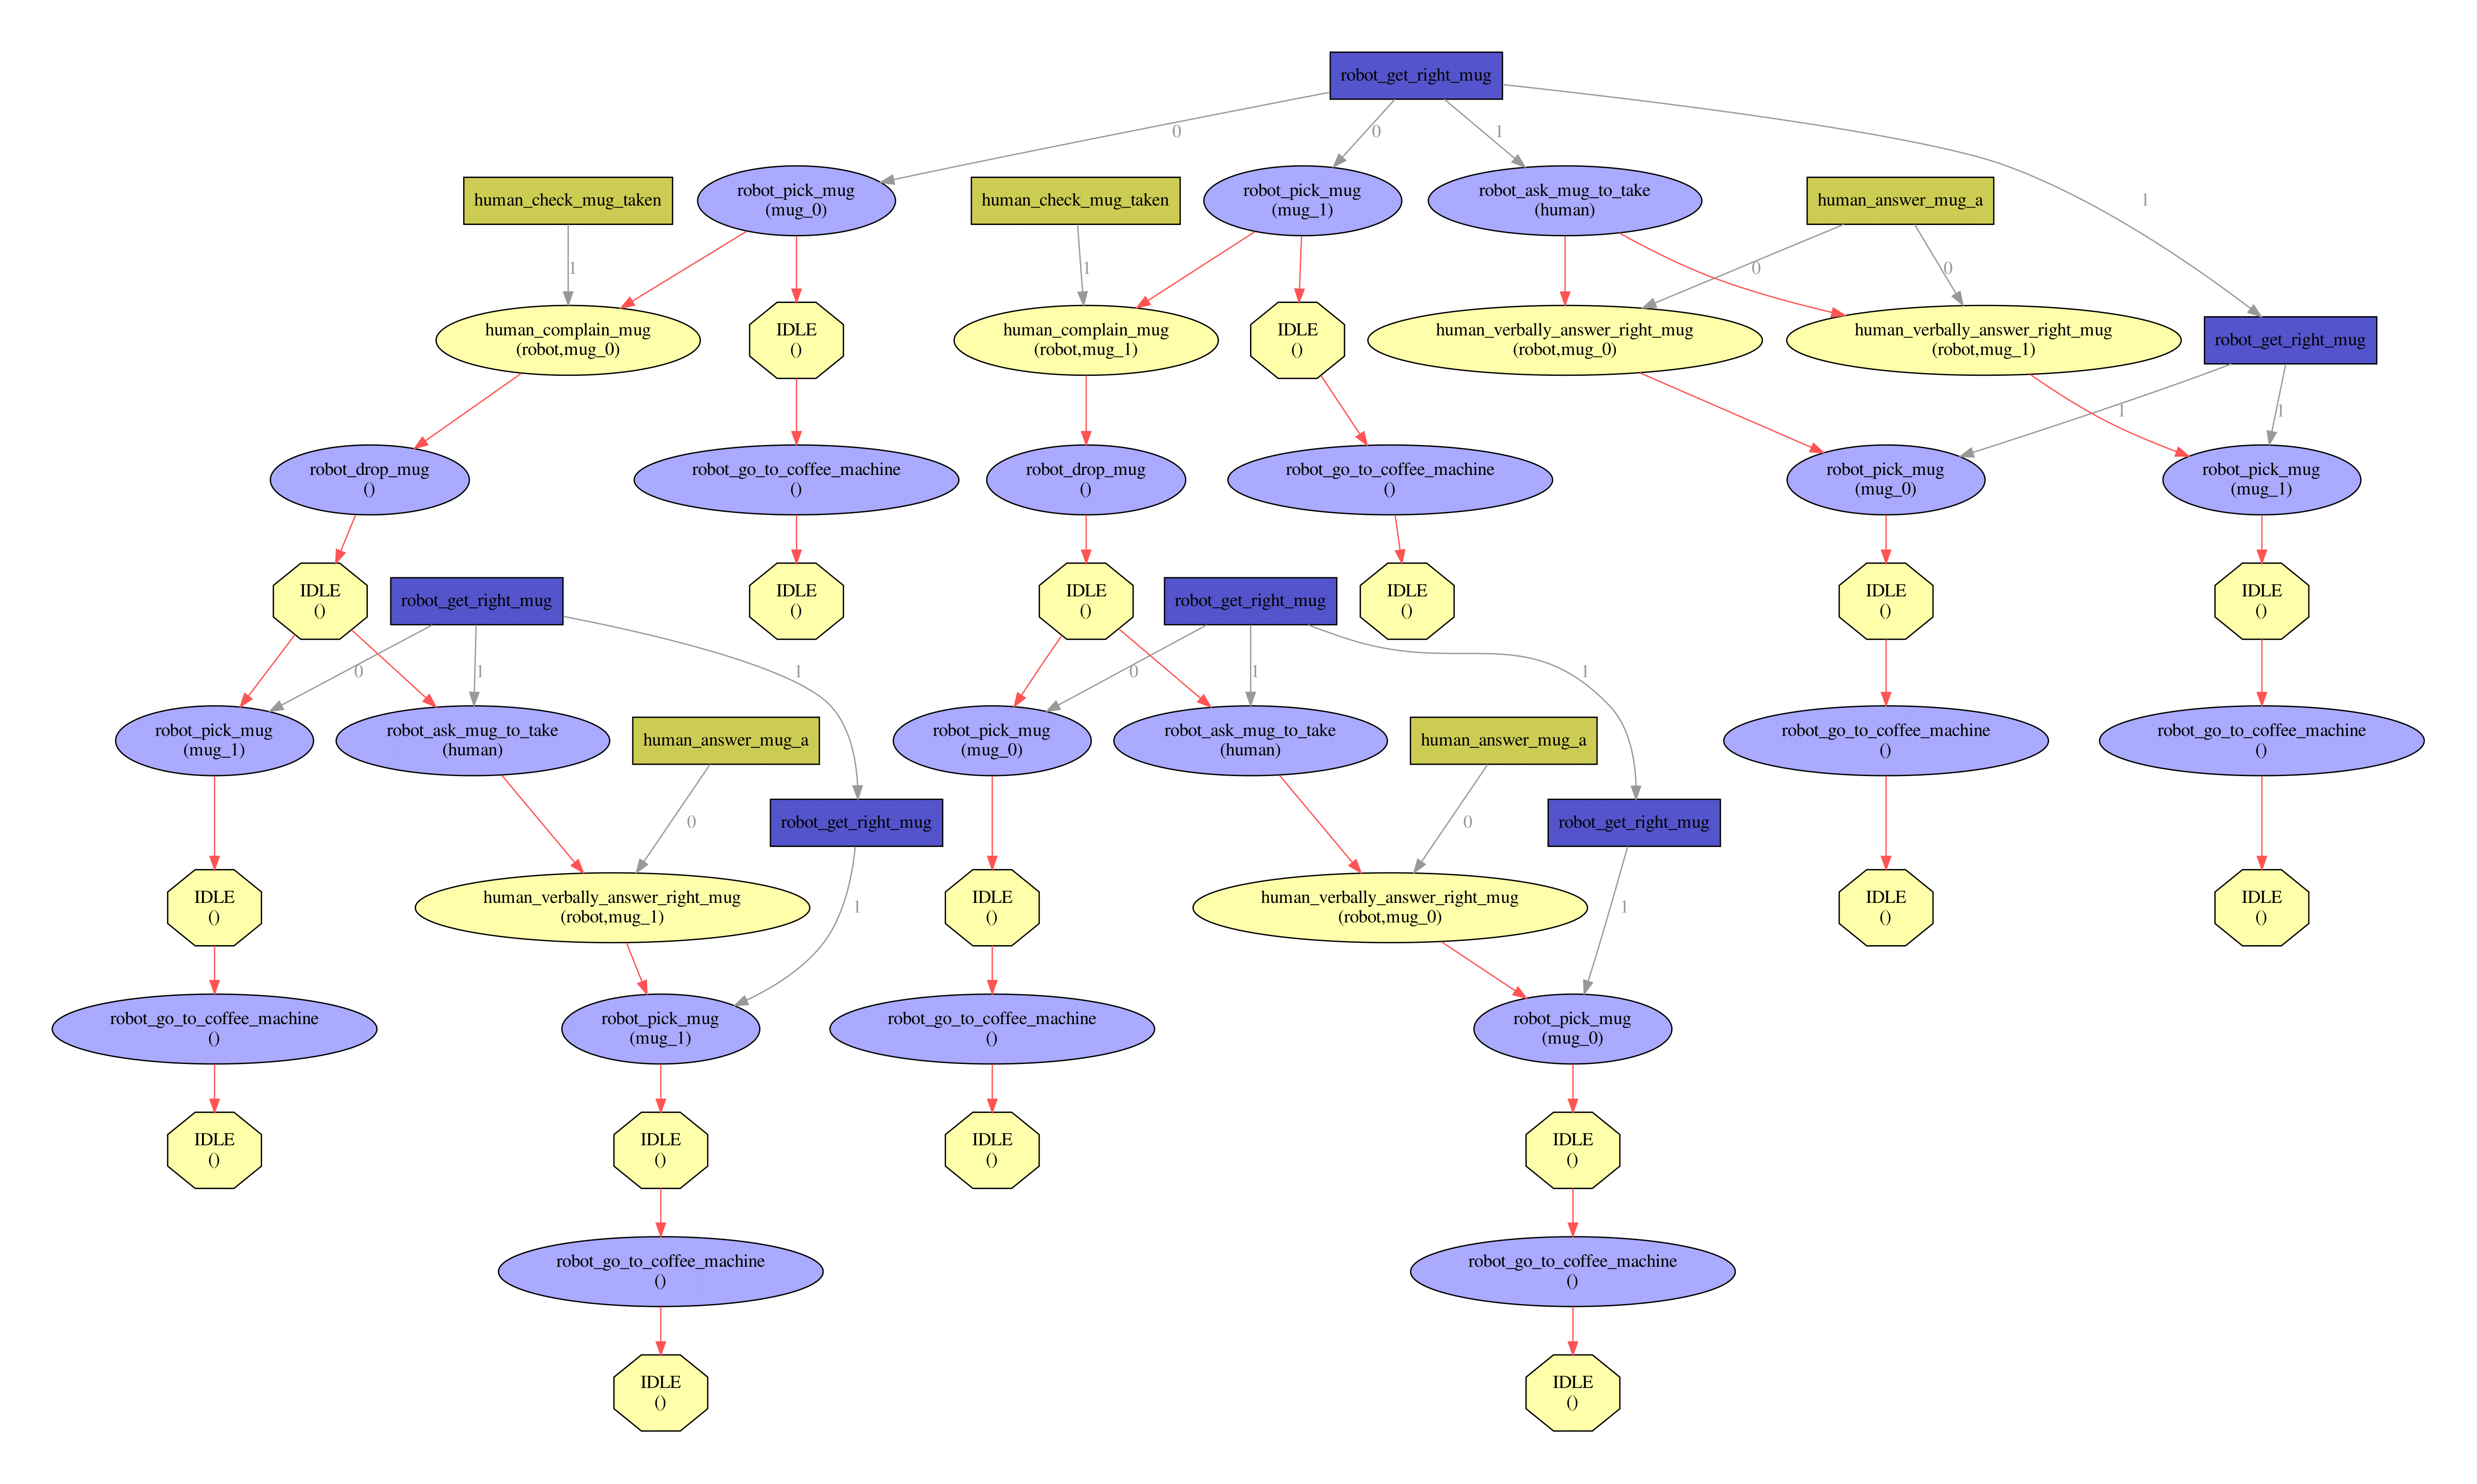
\includegraphics[width=\textwidth]{figures/chapter4/mug_selection_search_space.png}
\caption{CAPTION TODO}
\label{fig:chap4mugsss}
\end{figure}
\improvement{where can I introduce how to read this graph?}

The search space for $n=2$ mugs is presented in Figure~\ref{fig:chap4mugsss}. In this example, both mugs are distinct and RE can be computed. On the right hand side of the figure is the decomposition where the robot explicitly asks the human to designate her mug. The answer can either be \verb'mug_0' or \verb'mug_1'. The robot then pick the right one and go to the coffee machine, leaving no task to decompose.
On the left hand side of the figure is the decomposition where the robot proceeds via trials and errors. The robot can either pick \verb'mug_0' or \verb'mug_1' and the human will either react by doing nothing (if the robot took the right mug) or by complaining, in which case the robot will drop the mug, take the other one, and leave. Interestingly, we model the human reaction such as not expecting her to complain when taking the second mug after a first failure.

Next, we will compare different action costs and conditional plan selection criteria based on the same search space. To select a plan we used the Algorithm~\ref{alg:minaverage}. First, we set the cost of \verb'complain_mug' action much lower than the \verb'verbally_answer_right_mug' action. Here, the costs might have been set by the supervision component, estimating we are interacting in a noisy environment, where verbal communications are difficult to make, or that the human does not bother to correct the robot. The conditional plan returned is presented in Figure~\ref{fig:chap4mugtrialerror}. The chosen plan is the one containing trials and errors. Indeed, as it can lead to much shorter and thus less costly plans, it is the minimum average. 
\todo{caption}
\begin{figure}[hbtp]
\centering
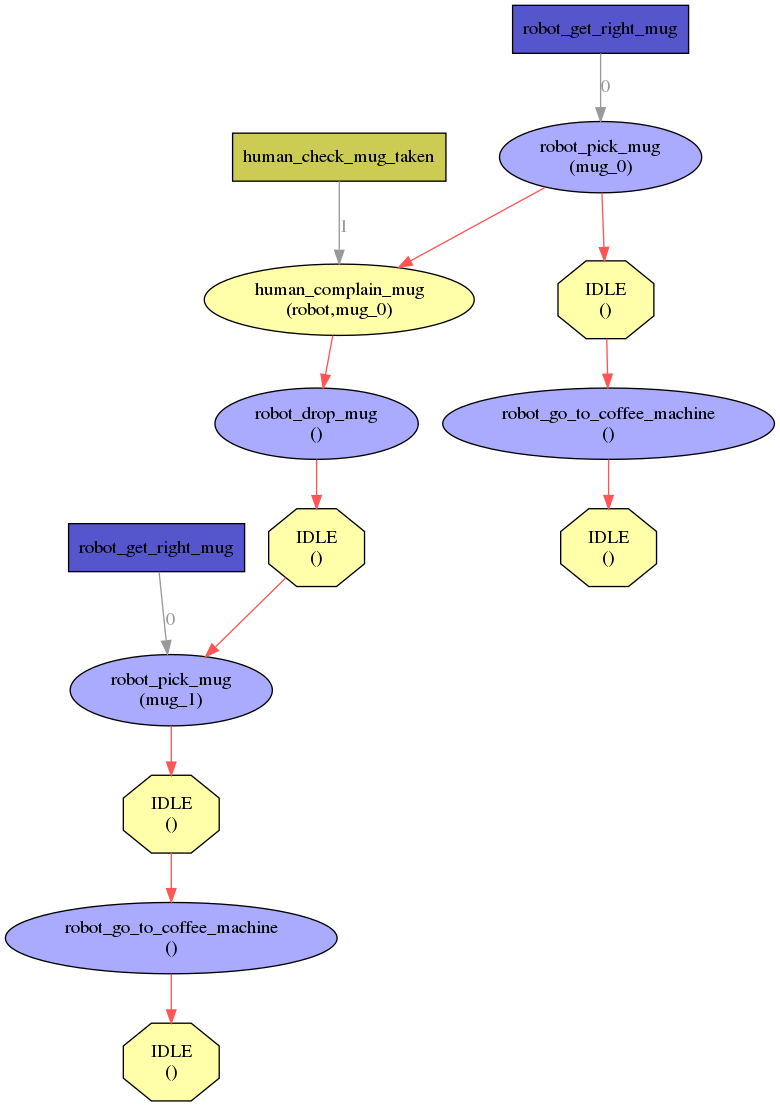
\includegraphics[width=0.8\textwidth]{figures/chapter4/mug_selection_trials.png}
\caption{CAPTION TODO}
\label{fig:chap4mugtrialerror}
\end{figure}

However, imagine that the human (who has still not had her coffee) is in a hurry, or that the mugs are really easy to distinguish from one another (\textit{e.g.} different color) and thus, we decrease the cost of the \verb'verbally_answer_right_mug' action and increase the cost of the \verb'complain_mug' action. The conditional plan selected is presented in Figure~\ref{fig:chap4mugask}. The robot know, prefers to ask for the right mug rather than trying to pick one at random.
\todo{caption}
\begin{figure}[hbtp]
\centering
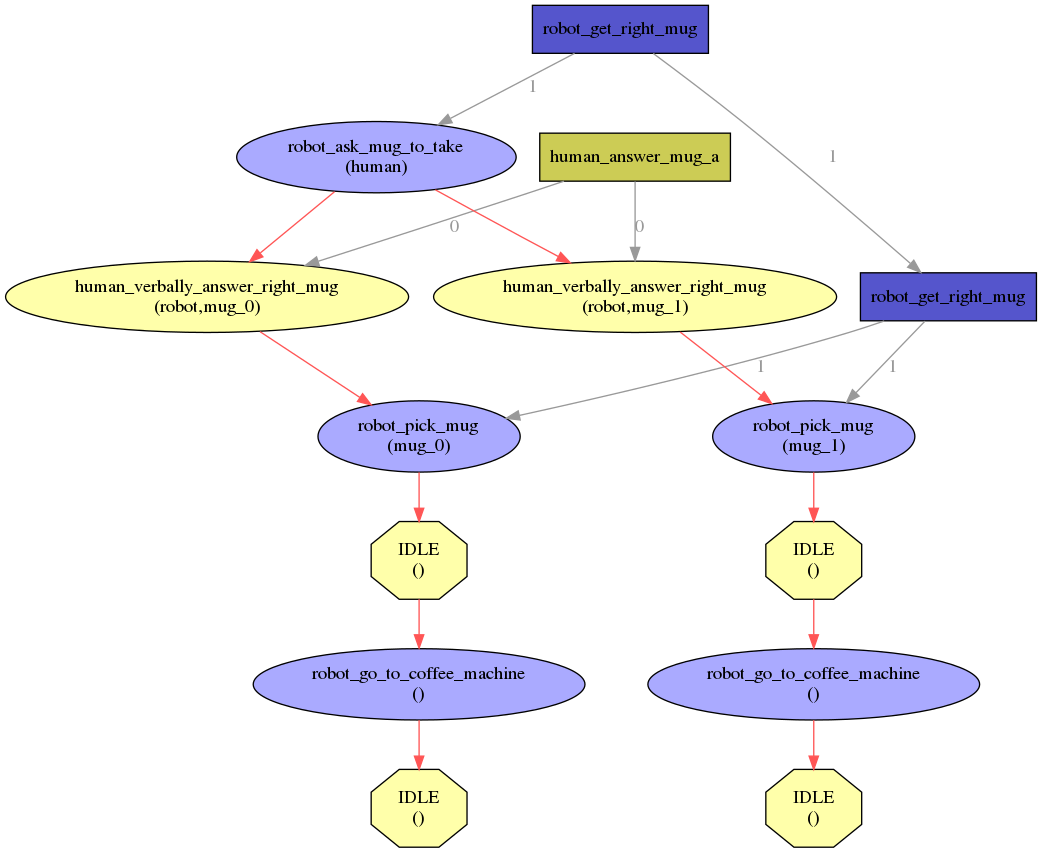
\includegraphics[width=\textwidth]{figures/chapter4/mug_selection_ask.png}
\caption{CAPTION TODO}
\label{fig:chap4mugask}
\end{figure}

As we increase the number of mugs $n$, the cost of \verb'verbally_answer_right_mug' has to also increase to make the robot choose the trials and errors decomposition, as the average of this decomposition increases since the number of potential errors increases. 
%Finally, if we make two mugs for which the REG does not find any solution (the mugs are not distinguishable from one another) the planner is able to generate conditional plans where it first tries to <-- not true for now, as we do not take into account failed actions in cost computation....

\improvement{Adds compute time for n=2,3,4,5}

\improvement{Add link to domain}

In this example we show one really interesting feature of our planner: representing human knowledge that is not known by the robot. While not being tractable when there are a lot of possibilities, it allows to select more or less conservative conditional plans depending on the cost of each actions. Moreover, this example allowed to see how updating the human agenda and how triggers can be used to model the agents interaction in the HTNs planning.
However, the human model was pretty simple, and we propose to challenge our planner in the next example with a task where the human is more involved.

\subsection{Balance difficult communications, decomposition cost and task attribution}
The robot is now heading to the coffee machine with the right mug in its gripper. On its way it detects another human taking a break near the coffee machine. The coffee has to be made. To brew coffee, ground coffee and water must be put in the coffee machine, and then the coffee can be served. While water is considered as always available, ground coffee is not. There are two places where ground coffee can be retrieved: either in the kitchen cupboard (close to the coffee machine) or in the pantry cupboard. 

\subsubsection{Handling the robot only case}
\label{subsubsec:chap4coffeerobotonly}
 First, we want the robot to be able to make coffee by itself, without requiring human help. To do so, we implement the following abstract tasks tree in the robot model (here we prepend the task names with \verb'r' where task are different in the robot and the human model):

\begin{itemize}
\item \verb'r_make_coffee' only having one decomposition (for now):
	\begin{itemize}
	\item \verb'r_make_coffee_alone' returning, in both orders (to represent partially ordered task tree), the tasks \verb'get_water', \verb'pour_water_in_machine' and \verb'r_get_coffee', \verb'put_coffee_in_machine'. Only \verb'r_get_coffee' is an abstract task.
	\end{itemize}
\item \verb'r_get_coffee' representing the ways for the robot to obtain coffee. It has only one decomposition:
	\begin{itemize}
	\item the decomposition returns $()$ if the robot has already coffee in its gripper. Else, it selects the closest cupboard and returns \verb'r_pick_coffee' with it as parameter.
	\end{itemize}
\end{itemize}

The robot primitive tasks as are follow:
\begin{itemize}
\item \verb'get_water' returning $\bot$ if the robot is already holding something; updating the beliefs of all the agents in the room with the fact that the robot holds water otherwise.
\item \verb'pour_water_in_machine' updating all the agents in the room beliefs with the machine being filled with water.
\item \verb'r_pick_coffee' returning $\bot$ if the robot is already holding something or if the cupboard passed as parameter does not contains coffee (in the robot beliefs); updating the beliefs of all agents in the room with the fact the the robot holds coffee otherwise.
\item \verb'put_coffee_in_machine' updating all the agents in the room beliefs with the machine being filled with coffee.
\item \verb'r_serve_coffee' updating all the agents in the room with the mug being filled with coffee.
\end{itemize}

Now, for the initial conditions we set that the robot knows there is coffee in the kitchen cupboard (the closest) and we add two tasks in its agenda: \verb'r_make_coffee' and \verb'r_serve_coffee'. The human has nothing in its agenda. The two possible plans for this really simple case are presented in Figure~\ref{fig:chap4coffeesimple}(a) and (b). The plan selection would then choose one of the plan based on robot action costs.

\todo{caption}
\begin{figure}[hbtp]
\centering
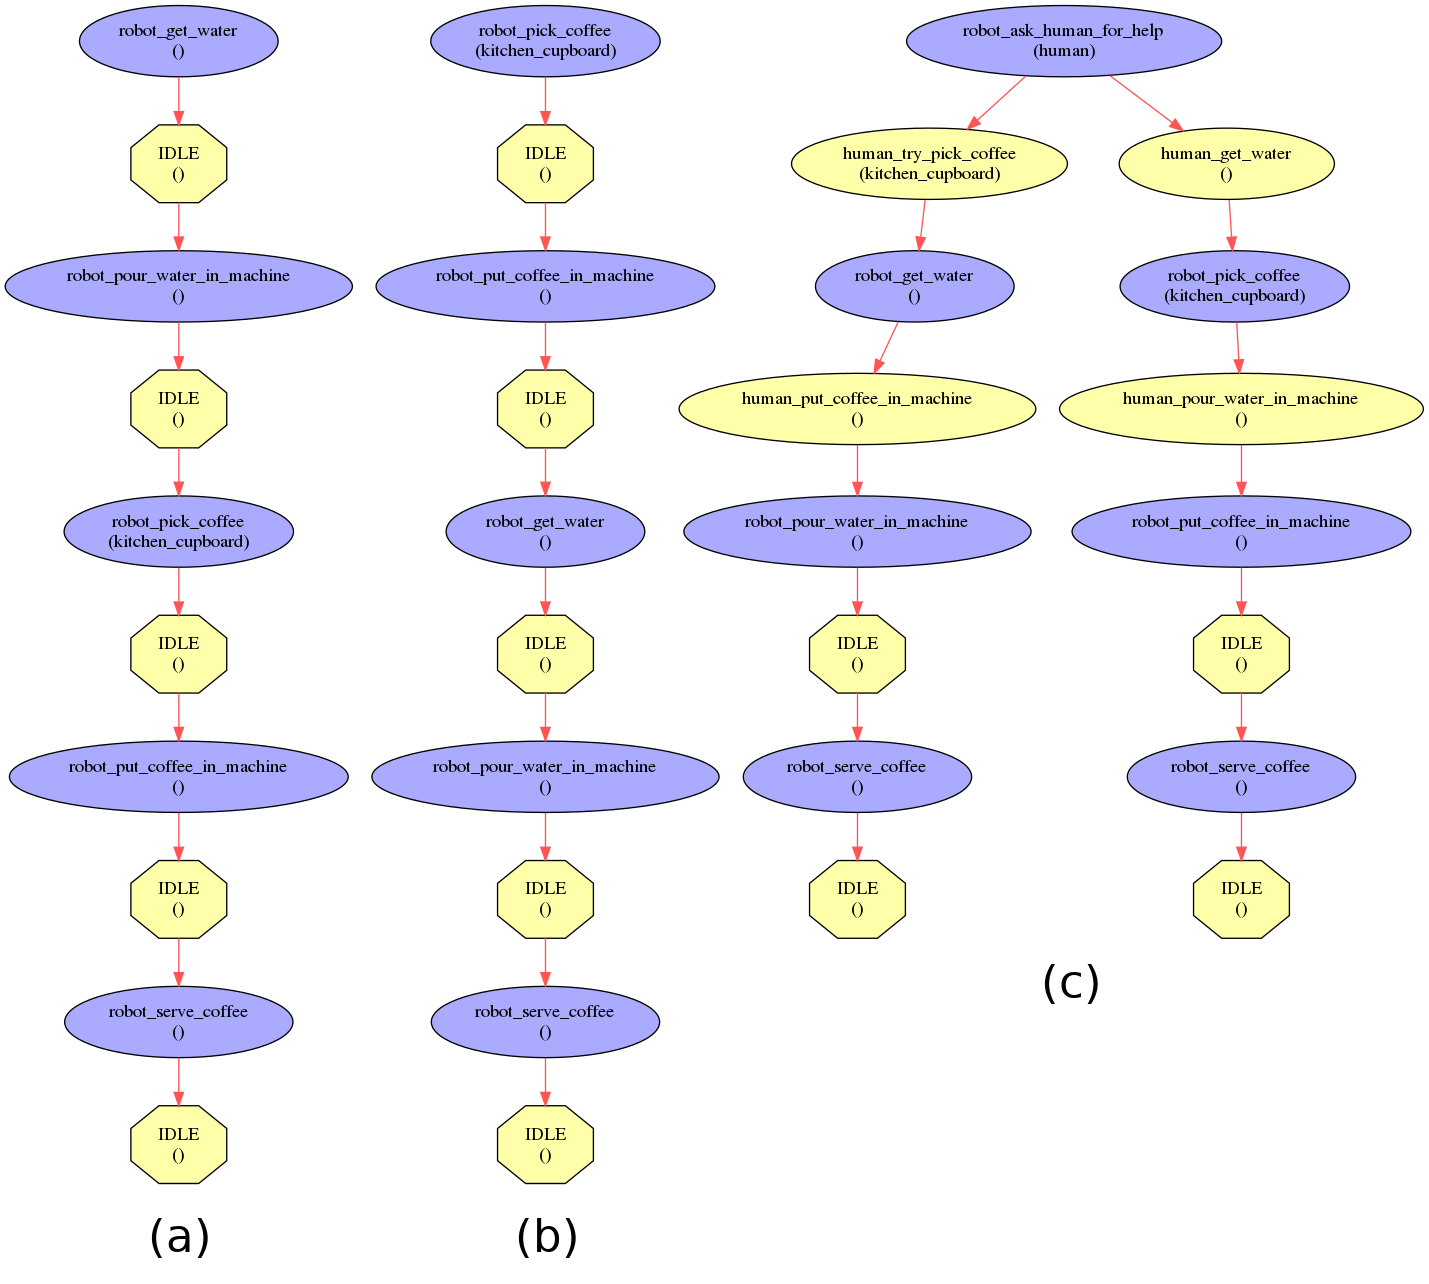
\includegraphics[width=\textwidth]{figures/chapter4/Chap4CoffeeSimplePlan.png}
\caption{CAPTION TODO}
\label{fig:chap4coffeesimple}
\end{figure}

\subsubsection{Incorporating the human planning process}
As we also want the robot to be able to ask the idling human to help it, we add, to its action model, a decomposition to the abstract task \verb'r_make_coffee' and a new abstract task \verb'help_make_coffee':

\begin{itemize}
\item \verb'r_make_coffee' containing the previous decomposition and the new one:
	\begin{itemize}
	\item \verb'r_make_coffee_collaboratively' returning the primitive task \verb'r_ask_human_for_help' and the abstract task \verb'r_help_make_coffee'
	\end{itemize}
\item \verb'help_make_coffee' representing the ways for the robot to help another agent to make coffee. It has only one decomposition:
	\begin{itemize}
	\item It returns \verb'get_water' and\verb'pour_water_in_machine' if there is no water in the machine and the human is doing a task related to bringing coffee. Likewise, it returns \verb'r_get_coffee' and \verb'put_coffee_in_machine' if there is no coffee in the machine and the human is doing a task related to fill the machine with water. Then, if the human is not doing any task, we add to the exploration \verb'r_get_coffee', \verb'put_coffee_in_machine' and \verb'help_make_coffee' if there is no coffee in the machine and \verb'get_water', \verb'pour_water_in_machine' and \verb'help_make_coffee'. The idea here is to complete the human actions if they take the initiative of a task, but to be proactive by exploring both possible alternatives if they are not. The recursion allows to reevaluate the need of this task later in the planning process.
	\end{itemize}
\end{itemize}

The primitive action added to the robot model is:
\begin{itemize}
\item \verb'r_ask_human_for_help' adding the task \verb'help_make_coffee' to the human agenda. Here we could have represented the possible refusal of the human by adding an abstract task leading to two possible decomposition for the human, accepting or declining, leading in similar schemes as in \ref{subsubsec:chap4coffeerobotonly}. However, to keep this example as simple as possible, we assume the human will always help the robot if asked to do so.
\end{itemize}

We model the human actions similarly to the robot ones. Their primitive tasks are defined as:
\begin{itemize}
\item \verb'help_make_coffee' representing the ways for the human to help another agent to make coffee. It has only one decomposition, which is the same as the robot one.
\item \verb'h_get_coffee' representing the ways for the human to obtain coffee. It has only one decomposition:
	\begin{itemize}
	\item the decomposition returns $()$ if the human is already holding coffee. Else, it selects the closest cupboard and returns \verb'h_try_pick_coffee' with it as parameter and \verb'h_get_coffee'. It differs from the robot one, indeed, whereas the knowledge of the robot is assumed to be the world state, the human's one can be false. Thus, the human might try to perform \verb'h_try_pick_coffee' on a cupboard not containing coffee. We take this into account with the recursion of this abstract task, and with the primitive task \verb'h_try_pick_coffee' described hereafter.
	\end{itemize}
\end{itemize}

The model of the human primitive actions are:
\begin{itemize}
\item \verb'get_water' as defined for the robot
\item \verb'pour_water_in_machine' as defined for the robot
\item \verb'h_try_pick_coffee' differs from the one defined for the robot as it checks if the cupboard passed as parameter really contains coffee (\textit{i.e.} in the robot beliefs). If it does not, the human's beliefs about this cupboard are updated to match the robot ones (modeling the human going in front of the cupboard, opening it and seeing the absence of coffee). If the cupboard does contain coffee in the robot beliefs, all the agents in the room beliefs are updated with the human having coffee in their hand.
\item \verb'put_coffee_in_machine' as defined for the robot.
\end{itemize}

The initial conditions are the same as presented before, but we also add that the kitchen cupboard contains coffee in the human beliefs. In addition to the two plans where the robot does not seek help to the human, another valid plan is found. This plan is presented in Figure~\ref{fig:chap4coffeesimple}(c). This conditional plan has two alternatives, depending on the initiative taken by the human.

\subsubsection{Updating human beliefs}
We can also change the initial conditions to elicit new behaviors. We keep the same action models for both the robot and the human, but we change the estimation of the human beliefs given as initial conditions to the planner. In a real robotic architecture, the human knowledge base would be updated with an estimation provided by situation assessment components. We specify that the human believes that both the kitchen and the pantry cupboard contain coffee. However, the robot knows (\textit{e.g.} using specific sensors or having been told about) that there is coffee only in the pantry cupboard. With these conditions, the search space extends to the three plans presented in Figure~\ref{fig:chap4coffeesimple}(a), (b), being when the robot prepare the coffee by itself, and in Figure~\ref{fig:chap4beliefsdiv}(a). In this last plan, we indeed model that the human will tend to first go to the nearest cupboard he thinks contains coffee. If this cupboard does not contain coffee, he will go to the next one. We can also note that only the left branch of the plan in Figure~\ref{fig:chap4beliefsdiv}(a) is impacted by this beliefs divergence. However, this branch choice is not up to the robot without any communication as we modeled the human as having the initiative of selecting a task. This subtlety cannot be represented in HATP.

Depending on the cost of the human being deceived and of the actions, the plan selected can be that the robot does all the task, as the human "mistake" can increase too much the average cost.

\todo{caption}
\begin{figure}[hbtp]
\centering
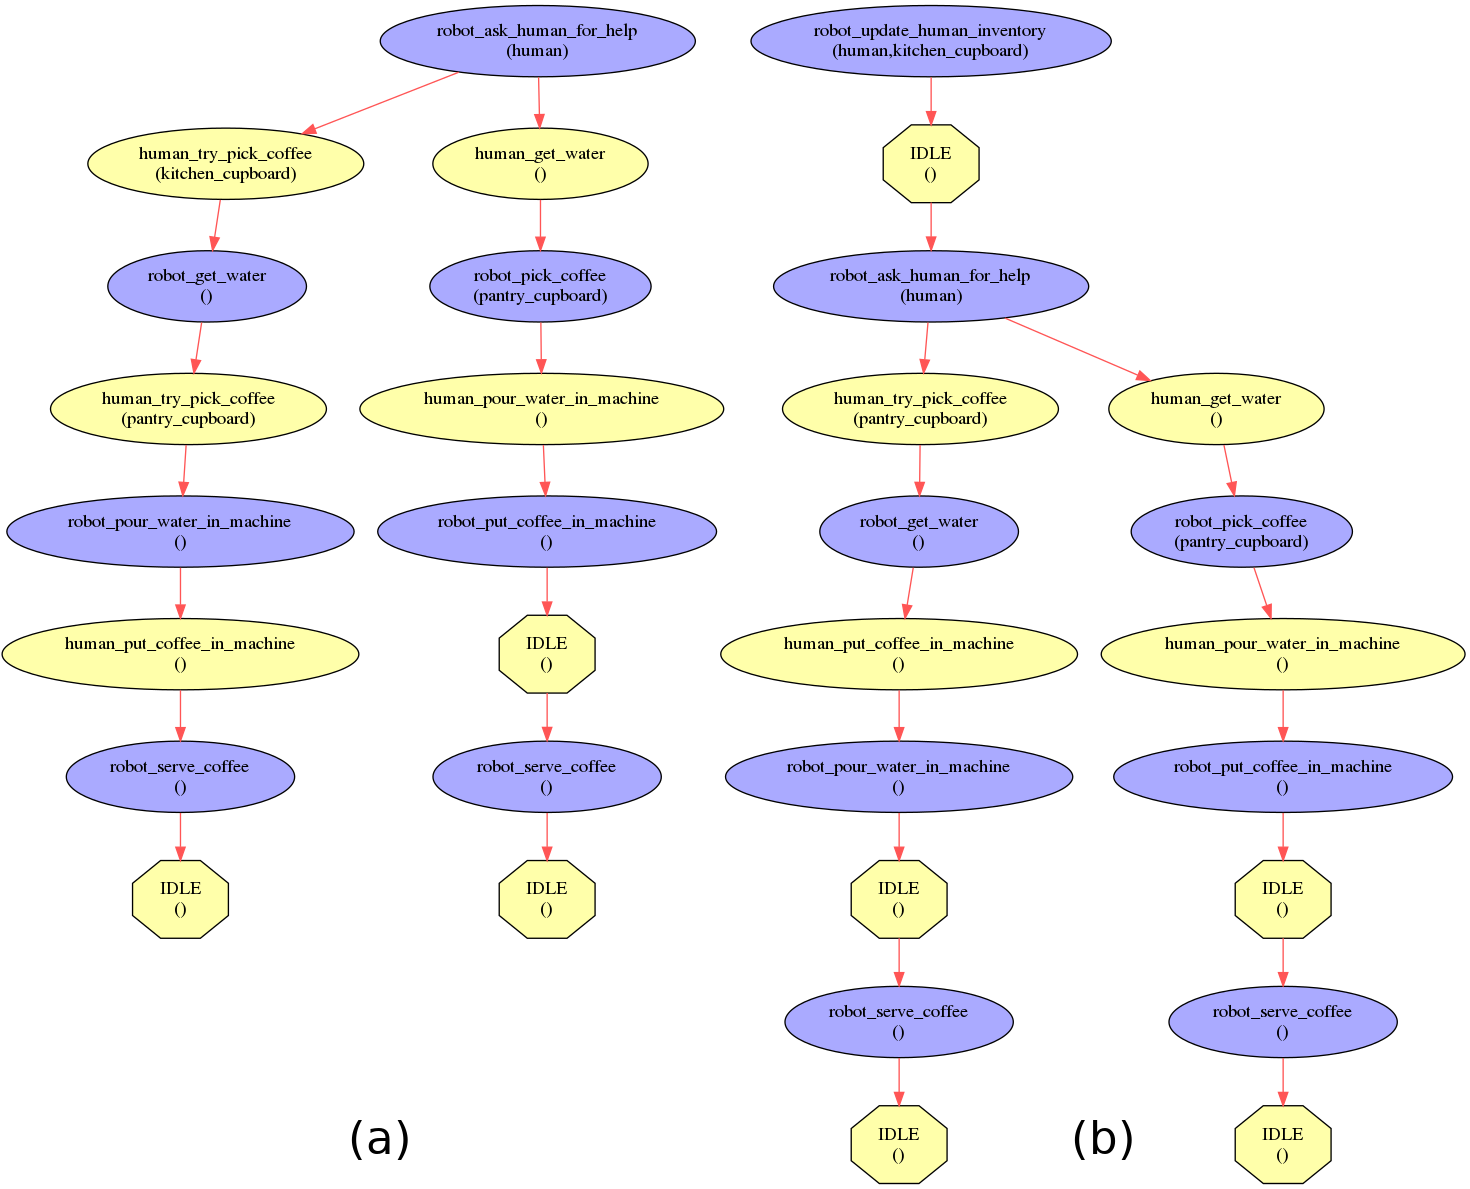
\includegraphics[width=\textwidth]{figures/chapter4/Chap4CoffeeBeliefDiv.png}
\caption{CAPTION TODO}
\label{fig:chap4beliefsdiv}
\end{figure}

To improve our robot, we want to make it able to realign the beliefs of the human, so, whatever the task he chooses, he will not make a mistake. To do so, we add a third decomposition to the \verb'r_make_coffee' abstract task and one new primitive task to the robot models.
\begin{itemize}
\item \verb'r_make_coffee' containing the previous two decompositions and the new one:
	\begin{itemize}
	\item \verb'r_align_and_make_coffee_collaboratively' returning $\bot$ if no belief divergence is detected between the robot and the human. The decomposition returns the new primitive task \verb'r_update_human_inventory' along with \verb'r_ask_human_for_help' and \verb'r_help_make_coffee'. An alternative for \verb'r_update_human_inventory' is returned with as parameter each cupboard in diverging beliefs between the robot and the human.
	\end{itemize}
\item \verb'r_update_human_inventory' being a primitive task. It updates the human beliefs concerning the cupboard passed as parameter with the beliefs of the robot.
\end{itemize}

With this new decomposition the new plan presented in Figure~\ref{fig:chap4beliefsdiv}(b) is added to the search space. In this plan the human beliefs are updated before asking him to help the robot to make coffee. The human does not make the mistake of going first to the kitchen cupboard.

Depending on the communication cost (estimated using the REG approach presented in the previous chapter), the human deception cost and the other actions costs any one of the four possible plans can be selected. For example, to minimize the human involvement and if the communication has a high cost, the selected plan would be Figure~\ref{fig:chap4coffeesimple}(a) or (b). If the communication is costly but the pantry and kitchen cupboard are not too far away, the selected plan is Figure~\ref{fig:chap4beliefsdiv}(a), finally, if we represent that the human would be upset if he makes a mistake or if the communication for aligning beliefs is not expensive, the plan Figure~\ref{fig:chap4beliefsdiv}(b) would be returned.

Through all these examples we show that this task planning approach, which separates human and robot beliefs and action models, can be suitable for multiple problems. We are able to plan for robot unknown human beliefs, to rely on the human planning process while keeping inherent uncertainties (\textit{i.e.} not making choices for them, without communicating them) and also to plan diverging beliefs and balance the actions of realigning them with plans containing mistakes. In the next section, we present a HRI task, inspired from psychology, that has never been tackled in robotics and we show how our planner is integrated in a fully functional robotic architecture dedicated for this task.


\section{The Director Task}
This work has been made in close collaboration with two other PhD. students Amandine Mayima and Guillaume Sarthou. 
\unsure{Dire qu'il y a un papier ?}

\subsection{A task used in psychology}
The director task is an experiment setup largely used and derived in psychology. It places two agents, the director and the receiver, in front of each other with a shelf in between. Usually, only the receiver is the participant, and the director is either an accomplice or a remote controlled agent (for computer-based experiment). The shelf consists in several compartments possibly containing objects. Each compartment can either be open on both opposite faces or open on only the receiver's side (hiding any contained object from the director, and being obvious for the receiver that the director cannot see inside it).

\todo{caption}
\begin{figure}[hbtp]
\centering
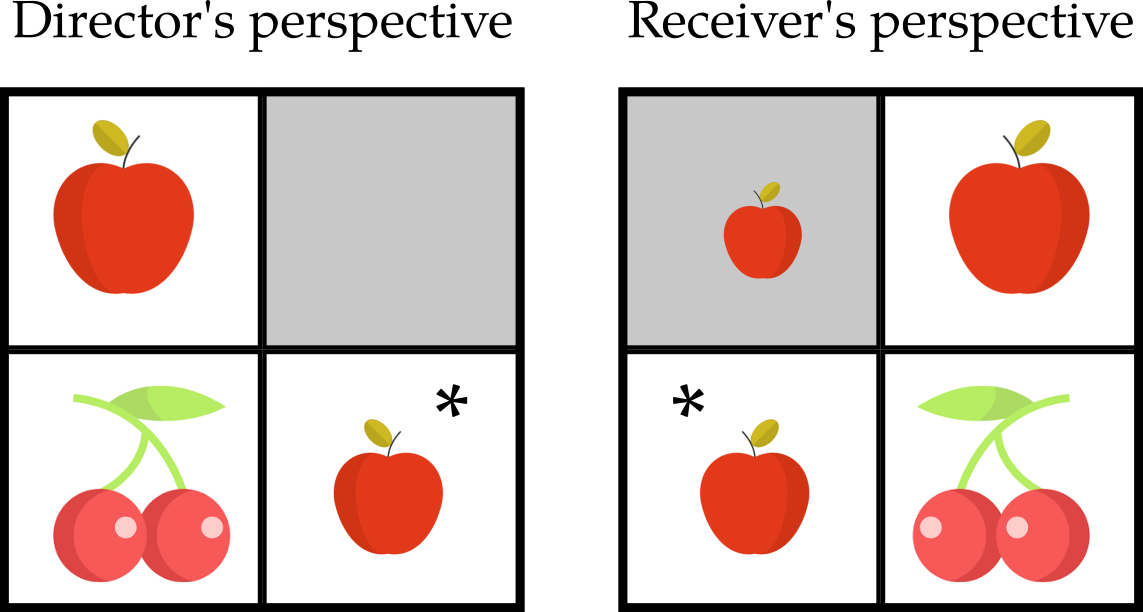
\includegraphics[width=\textwidth]{figures/chapter4/dt_apple.png}
\caption{CAPTION TODO}
\label{fig:chap4dtapple}
\end{figure}

The director asks the receiver to move some objects by describing them. However, some descriptions of the director will also match other objects ---called competitors--- that are only visible by the receiver (Figure~\ref{fig:chap4dtapple}). Hence, the receiver must think that the object matching the description cannot be the one referred by the director as they are not aware of it, and find the object matching the description in the director's beliefs. This process must then be maintained all along the interaction as the situation evolves.

This task is used in psychology to study how perspective-taking is used for communication understanding while performing a task with another agent \cite{keysar2000taking}. Results show that, even if the receiver considered or took a competitor for the first trial, they are able to take the one designated by the director during subsequent trials. This shows that even if participants understand language in an egocentric way, they are able to do perspective-taking to successfully perform the task \cite{keysar2003limits}. 

Even if this task is well known by psychologists, to our knowledge, no robot managed to handle it. A robot that does would prove its architecture being able to maintain self-other distinction of beliefs but also to perform perspective taking on its human partner. We propose a robotic architecture integrating our planner, that is able to handle both side of the director task. Besides, we propose some changes for both the director and receiver roles to be interesting along with planning challenges some modifications of the task can arise.

\subsection{Setup}
The setup we propose is a slight variation of the original director task used in psychology. First, instead of moving objects between compartments, the high level known goal is to remove a subset of the objects in the compartments and to place them in a receiver accessible only area (on top of a table). 
Then, objects are replaced with blocks having four special attributes: their color, the color of their border, the shape drawn on them and the color of this shape. The colors can either be blue or green, and the shapes either a triangle or a circle. This allows for a maximum of ambiguity between the blocks. 
Besides, to make the task interesting for both the director and receiver roles, compartment are not only either fully opened or hiding content from the director, they can also be hiding content from the receiver while being opened towards the director. Thus, not only the receiver must take the perspective of the director to understand the right block, but the director has also to take the perspective of the receiver to make the smallest instruction possible to respect the maxim of quantity~\cite{grice1975logic}.
In addition, to increase the number of ambiguous situations, we prohibit the use of geometrical relations during the communications (\textit{e.g.} "the leftmost block", "the block above the green one") to only allow the use of the block attributes. Likewise, pointing at a block is forbidden.
Finally, every blocks and compartments are equipped with AR-tags (different on each face) allowing the robot to easily detect them and to make an accurate representation of the environment.

\subsection{The robotic architecture}
The robotic architecture is composed of several elements.
First, the knowledge base chosen is an ontology. As we have shown before, ontologies are more and more common in robotics as they allow for rich and complete reasoning mechanisms and efficient requests of symbolic facts. The software used is \textit{Ontologenius}~\cite{sarthou2019ontologenius}. An ontology is created for the robot ($\robotmodel$, which we use as the true state of the environment) and another one is created for the human ($\humanmodel$) representing the robot estimation of the human knowledge. As stated in the previous chapter, these ontologies can be queried or updated through an efficient low-level API or higher-level \sparql{} queries. The interfaces between the ontologies and our planner are presented in \ref{subsec:chap4integratingwithothers}. The ontology is initialized with static facts being (1) the link between each AR-tag and their matching block and compartment, (2) the attributes of each block, (3) the 3D models of each block and compartment.

To gather all the robot sensing data, create a geometric representation of the environment, compute symbolic facts from it for both the robot and the human and update the ontologies with them, a situation assessment component is added to the architecture. This component is based on underwolds~\cite{lemaignan2018underworlds} allowing for modular and reusable reasoners. It first gathers the data from perception algorithm (AR-tags positions for the objects and motion capture for the human), then creates a geometrical scene of the environment. Based on it, the component is able to compute symbolic facts: \textit{isIn}, \textit{isVisibleBy}, \textit{isReachableBy}, \textit{isOnTopOf}; and feed them in real time to the ontology. This component also estimates the geometrical scene viewed and known by the human, computes symbolic facts on it and feed the corresponding ontology.

Then, to be able to give and understand instructions, the REG component presented in the previous chapter is also included. A grammar-based verbalization component allows to transform the generated RE into natural language. Similarly, a natural language request can be interpreted as a \sparql{} query and matched against an ontology.

To orchestrate all the components, the supervision system called JAHRVIS (Joint Action-based Human-aware supeRVISor) is dedicated to manage the interaction. It not only handles the robot actions but also estimates the human mental state, monitors the human actions and manages the communication with them. It manages five facets of the interaction: (1) interactions sessions, (2) communication, (3) human, (4) task and (5) quality of interaction. It is responsible for task planning requests and plan execution and monitoring.

Finally, the task planning component used in this architecture is the one presented in this chapter. Task planning is only required when the robot is the director, since when the robot is receiver it only has to execute commanded instructions. When the robot is the director, the supervision system is given a list of blocks (via their ids) to remove from the shelves. This list is then passed as the goal parameter of a task to decompose to the planner.
The task to decompose is called \verb'clear_blocks' and is filled with a parameter representing the goal and another being the human id. The goal is simply an under specified world state, composed of triplets containing for example \verb'(block_23, isIn, disposalArea)'.
The robot task planning domain ($\robotmodel$) is presented hereafter. 
\begin{itemize}
\item The \verb'clear_blocks' abstract task has only one (recursive) decomposition. The decomposition returns $()$ if the blocks specified in the goal matches the relations also specified in the goal. Otherwise, a REG request is performed for all the misplaced blocks, and the tasks \verb'clear_one_block' and \verb'clear_blocks' are returned, with the easiest block to refer to (\textit{i.e.} lowest RE cost) as parameter of the \verb'clear_one_block' task.
\item The \verb'clear_one_block' task has also only one decomposition returning the primitive task \verb'tell_human_to_clear_block' and the abstract one \verb'wait_for_human_to_clear_block'.
\item The \verb'wait_for_human_to_clear_block' abstract task has only one decomposition. It aims at recursively planning to wait until we planned the human has removed and put the right block away. It recursively decomposes into $()$ if the block passed as argument is in the right place; and returns \verb'wait' and \verb'wait_for_human_to_clear_block' otherwise.
\end{itemize}

The robot primitive tasks are defined as follow:
\begin{itemize}
\item The \verb'tell_human_to_clear_block' primitive task returns $\bot$ if the block specified as parameter is not reachable by the human, or if it is not present in the human beliefs $\humanmodel$. Else, it adds the abstract task \verb'clear_told_block' to the human agenda passing the specified block as parameter and does not update any beliefs.
\item The \verb'wait' primitive task does not update any beliefs.
\end{itemize}

On the human tasks side, we modeled a cooperative human, non declining asked tasks. Thus, the task model is as follows:
\begin{itemize}
\item The abstract task \verb'clear_told_block' has only one decomposition, returning the primitive tasks \verb'pick_block' and \verb'place_block'.
\item The primitive task \verb'pick_block' return $\bot$ if the block passed as parameter is not reachable by the human in their beliefs; and updates the beliefs of all the agents in the room with the human holding the block otherwise.
\item The primitive task \verb'place_block' return $\bot$ if the human is not carrying anything; else it updates the beliefs of all the agents in the room with the block being placed in the area specified as parameter, and the human not holding anything.
\end{itemize}

In the domain described previously, we compute in the abstract task the least costly block to refer to to decompose the task. This greedy approach can be used because we remove the block during the task. The referring cost of blocks thus can only decrease at each iteration of the task. However, it would be completely different if some blocks were to be added to the shelf along with others to remove. There, our greedy approach would not work as an not costly action would make future actions more costly leading to an sub-optimal plan. Another approach could be to have the decomposition of \verb'clear_blocks' to return all the orders of the block removing instructions to explore.

In the proposed version of the director task, only the cube order can be planned. Thus, in the following subsection, we propose slight variations of the task increasing the planning complexity and interest, along with some possible modeling directions to overcome these challenges.

\subsection{Challenges for planning}
To spice up the planning challenge in the director task, we propose some extensions to the presented task.
First, by adding blocks with identical visual features to the shelf, and asking to remove a precise one of them, we introduce situations where verbal communication (and REG) is not enough to refer to a block. To solve this problem, we could for example add a decomposition to \verb'clear_one_block'. In this decomposition, we could have the robot moving one distractor of the REG in a non visible compartment to be able to refer to the intended block. The planner would then have to balance between making the referring easier by moving a block before giving the instruction and giving a long and complex instruction (when feasible).

With the same scenario, using the REG extension presented in the previous chapter, allowing the RE to contain relations to past common actions, we could introduce another way for the robot to refer to a block. The planner would need to balance previous communication means with creating a unique past experience with a block to easily refer to it (\textit{e.g.} "the blue block that I just moved").

Besides, we can add multiple distinct disposal areas for blocks. The director would then have to instruct the receiver not only the block to pick but also which area they have to place it in. Furthermore, we could also add a decomposition where the robot ask to pick an under specified block, ensuring that all the matching ones need to be removed, and plan for all the possible blocks picked by the human matching this description. Depending on the block picked, it would be planned to ask to place the cube in its corresponding area. This may result in a better efficiency as it would lead to less complex referring expressions.

Finally, performing this task will necessarily bring errors, either from the human (\textit{e.g.} the wrong block may be picked) or the robot (\textit{e.g.} a block may fail to be picked). Even if some errors can be planned for (\textit{e.g.} modeling all the blocks the human can pick and planning accordingly) doing so for all the possible contingencies is not possible. Therefore, a strong link with supervision must be envisioned as it will ask for replanning. Replanning is not as simple as passing the current state and the same goal and starting the process all over again, since some task decomposition may have been executed partially and cannot be changed in the replanning process.

% Code words + Multiple sessions
% Communicating about multiple blocks at once

\section{Conclusion and Future Works}
In this chapter we proposed a new task planning approach for human robot interaction. This approach not only explicitly represent and plan upon both the human and the robot beliefs but also use two separate action models as HTNs for the human and the robot.

We proposed a formalism along with an algorithm allowing to plan for robot actions, while considering the possible human actions according to their task model. By doing so, we are able to represent and to account for the human planning and reaction processes.

Then, we presented a successful implementation of this approach in Python and showed first results along two examples. These examples highlighted both the features of the prototype planner and the rationale behind the action models crafting. The planer is able to represent and to plan for robot unknown human knowledge, human reactions to robot actions, multiple human possible plans and intricate human robot tasks. It is also capable of balancing between communicating, letting the human perform a mistake and attributing different roles to the robot or the human.

Finally, we introduced a simple to reproduce while challenging collaborative task inspired from psychology studies: the director task. To be performed by a robot, this task includes several prerequisites such as being able to take the perspective of the human partner and to refer objects in a dynamically evolving environment. The robot architecture built to handle the task allowed us to show how our prototype planner can be used on a real task in a complete robotic architecture. Some extensions of this task challenging for task planning were introduced along with hints to complete them.

We look forward to continue exploring this approach, find its benefits and its limits. More importantly we aspire at improving it, especially on the following topics.

\subsection{Representing explicitly observation processes}
A lot of code is common between the primitive tasks not only in a planning domain but also between multiple ones. Indeed, the part where we update the beliefs of the agent performing the action, but also the ones of the other agents in the room is present in almost all the primitive actions. This commonality raises the question of observability of actions. Indeed, even if we can assume that when an agent is planned to do an action they will be aware of its effects, and that if the human is planned to perform an action, even if it is not observable from the planned robot position, we update the beliefs of the robot (as it is emulating the human actions), it is not the case for a robot action and the update of human beliefs. We can represent is coarsely in the primitive task effects by relying on heuristics such as the presence of the agents in the same room. Still, observabilty of actions may need a specific representation for belief update in the planner core.

Besides, even if we plan that the human will do one action or the other at one point in the plan, recognizing and distinguishing between them may not be possible during the execution. This can endanger the interaction as the wrong branch of the plan may be executed. Thus, the supervision component must be informed, along with the plan, of the observability of the human actions, which can, in turn, impact the plan selection process.

%\subsection{Leveling-up the theory of mind}

\subsection{Pruning during the search space exploration}
For now, all the search space is explored to find valid plans, and only then the cost of actions are evaluated to select the optimal conditional plan. However, even if the search is guided by the HTNs, the branching factor can become large, especially if the planning process is executed in a robotic architecture while interacting with a human. Thus, it is possible to evaluate the plan cost during exploration and to prune some branches in the search space according to the best plan found so far. Yet, doing so would prevent from applying plan wide costs, as they could change the optimality of the plan used during in the search.

Another approach would be to learn which actions a human is more likely to perform in a certain state. We could then prune all the least probable human actions (still returned by their modeled task tree). Although this approach can be easy to implement, learning must be done per human (as two humans may react differently in the same situation) and on a few learning samples as the same world state seldom appears during specific tasks on typical short term laboratory scenarios and generalization could be difficult.

Finally, we can also imagine that the robot might ask the human which tasks they are likely to perform at a specific step in the plan, while elaborating the plan. This would lead to negotiations with the human making the final plan more acceptable while also reducing the branching factor as only the tasks answered by the human would be explored. However, for long and complex domains, this solution may confuse the human because it would require them to project on the long-term among multiple conditional eventualities.

\ifdefined\included
\else
\bibliographystyle{acm}
\bibliography{These}
\end{document}
\fi
